% The Klein bottle as a square: one pair of edges identified with a flip.
% Source: book/tex/topology/constructions.tex (§ The Klein bottle).
\documentclass[border=2mm]{standalone}
\usepackage{tikz}
\usetikzlibrary{arrows.meta,decorations.markings}
\tikzset{midarr/.style={decoration={markings,
  mark=at position 0.55 with {\arrow{Latex[length=2mm]}}},postaction={decorate}}}
\begin{document}
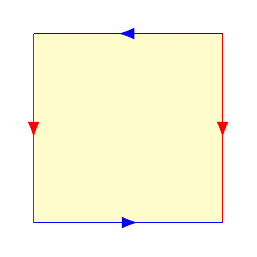
\begin{tikzpicture}[scale=2.4]
  \fill[yellow!20] (0,0) rectangle (1,1);
  % C=(0,0) B=(1,0) A=(1,1) D=(0,1)
  \draw[red, midarr]  (1,1) -- (1,0); % right edge, downward
  \draw[blue, midarr] (0,0) -- (1,0); % bottom edge, rightward (flipped)
  \draw[red, midarr]  (0,1) -- (0,0); % left edge, downward
  \draw[blue, midarr] (1,1) -- (0,1); % top edge, leftward
\end{tikzpicture}
\end{document}
